\documentclass[utf8]{beamer}

\usepackage{beamerthemesplit}
\usepackage{latexsym}
\usepackage{eurosym}
\usepackage[activeacute,spanish]{babel}
\usepackage{ae,aecompl}
\usepackage{graphicx}
\usepackage{amsfonts}


\mode<presentation>{
\usetheme{Warsaw}
\usecolortheme[RGB={148,20,110}]{structure}
\setbeamercovered{transparent}
}

\title{CONTROL DE GASTOS}
\subtitle {Proyecto del Primer Parcial}
\author{Vannesa Robles  Ricardo Campuzano  Ana Mora Ocaña}
\date{\today}
\institute {ESPOL}

\begin{document}
\begin{frame}[plain]{Lenguajes de programación}
\begin{center}

\includegraphics [width = 0.2 \textwidth]{logo.jpg} %para colocar el logo de la presentación
\end{center}
\titlepage
\end{frame}

%indice
\begin{frame}
\frametitle{Esquema} %Esquema es el titulo de la diapositiva
\tableofcontents[pausesections]
\end{frame}

\section{Problema a Resolver}
\begin{frame}[allowframebreaks]

\begin{block}{Problema a Resolver }
Actualmente,  hemos notado que a más de una persona que lleva una contabilidad para declarar sus impuestos en el SRI no sabe que hacer, esto se vuelve tormentoso a la hora de buscar facturas, saber cuanto gastos se ha realizado, recordar las fechas de declaración y por lo general las personas de poco conocimiento en el funcionamiento o manejo de esta entidad buscan contratar adicionalmente una persona que les realicen dicho proceso de llevar la contabilidad de sus actividades. Es este principal interés el que nos vemos en la necesidad de digitalizar dicha información de una manera màs facil para las personas natural que realizan esta actividad, la declaración de sus impuestos.
\end {block}
\end{frame}

\section{Objetivos}
\begin{frame}[allowframebreaks]

\begin{block}{Objetivos}
Actualmente,  hemos notado que a más de una persona que lleva una contabilidad para declarar sus impuestos en el SRI no sabe que hacer, esto se vuelve tormentoso a la hora de buscar facturas, saber cuanto gastos se ha realizado, recordar las fechas de declaración y por lo general las personas de poco conocimiento en el funcionamiento o manejo de esta entidad buscan contratar adicionalmente una persona que les realicen dicho proceso de llevar la contabilidad de sus actividades. Es este principal interés el que nos vemos en la necesidad de digitalizar dicha información de una manera màs facil para las personas natural que realizan esta actividad, la declaración de sus impuestos.
\end {block}
\end{frame}



\section{Descripción}

\begin{frame}[allowframebreaks]


\begin{block}{descripción de la Aplicación}

Esta aplicación ayudará al usuario a llevar un mejor control de sus facturas, clasificando cada ingreso de datos de las facturas en el tipo de gasto que corresponda, asi como tambien generando un reporte detallado. 
Facture SRI  ayudará  recordando la fecha máxima de entrega de el reporte al SRI. 
Mediante la automatización el sistema clasificará la información por número de RUC del proveedor y tipo de gasto generando los siguientes reportes: 
\end {block}

\end{frame}

\section{Aplicación}  
\begin{frame}[allowframbreaks]
\frametitle{Imagenes}
\begin{center}

\includegraphics[width=0.3\textwidth]{cargando.png}
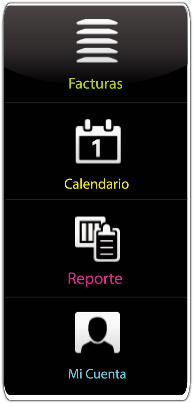
\includegraphics[width=0.3\textwidth]{menuprincipal.png}
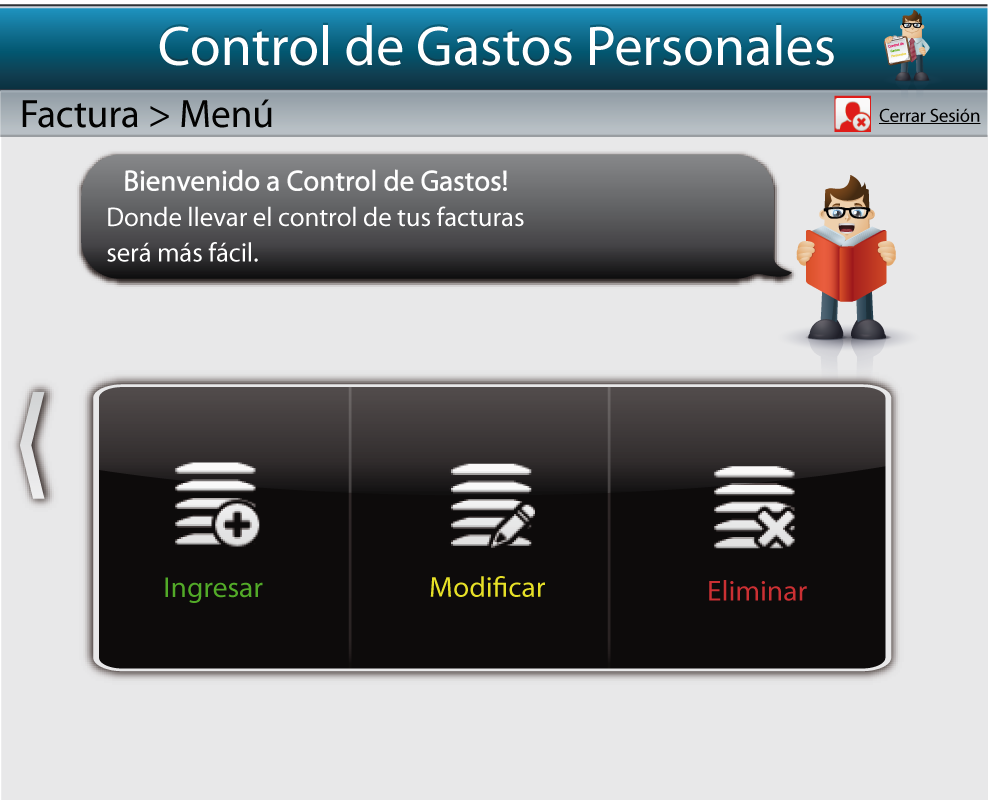
\includegraphics[width=0.3\textwidth]{factura.png}
\end{center}
\end{frame}

\begin{frame}[allowframbreaks]
\frametitle{Imagenes}
\begin{center}
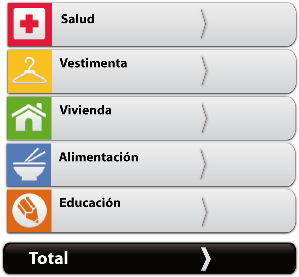
\includegraphics[width=0.3\textwidth]{informe_gastos.png}
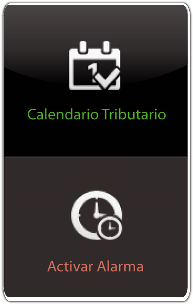
\includegraphics[width=0.3\textwidth]{alarma_over.png}
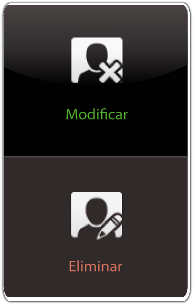
\includegraphics[width=0.3\textwidth]{micuentaelimi_over.png}
\end{center}
\end{frame}

\end{document}